\section{Experiments of the supervised approach} \label{supervised_approach_experiments}

We performed several experiments to optimize the parameters of the supervised approach. They are divided into three sections. First, three experiments regarding the architecture and training pipeline are performed. They test two different dropout rates, two sizes for the hidden layer and two different learning rate schedulers. The results of these three experiments are used in the following experiments.

The next row of experiments involve around the \acrfull{asl}, which replaces the \acrshort{bce} loss function that was used in previous experiments. Each experiment focuses on one of its two parameters, to find the best configuration for our use case.

Finally, the last experiment assesses the combination of the \acrshort{asl} and the \acrfull{mcl} for the coherent model, which is exactly the same as the one used in previous experiments, but which an additional layer on top, called the \acrlong{mcm}. Given that both the \acrshort{asl} and the \acrfull{mcl} extend the \acrshort{bce} loss function, we can combine them. We evaluate if doing so is more performant than the original loss function of the coherent model (the \acrshort{mcl}).

\subsection{Optimization experiments} \label{supervised_approach_optim}

Here we optimize several parameters, both of the model and of the training procedure. We do so by running experiments with two values we deem reasonable for each of these parameters. The parameters we consider are dropout probability, hidden layer size and scheduler.

\subsubsection{Dropout probability}

\begin{figure}
  \begin{subfigure}[t]{.5\textwidth}
    \centering
    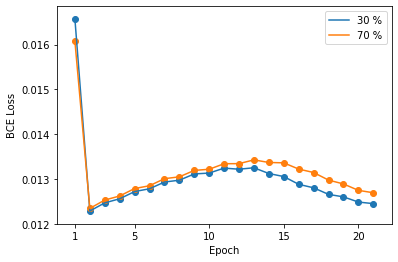
\includegraphics[width=\textwidth]{figures/supervised_approach/dropout_train_loss.png}
    \caption{Training loss}
    \label{fig:dropout_train_loss}
  \end{subfigure}
   \begin{subfigure}[t]{.5\textwidth}
    \centering
    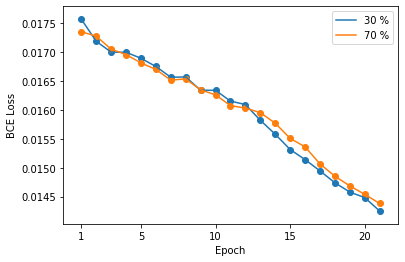
\includegraphics[width=\textwidth]{figures/supervised_approach/dropout_test_loss.png}
    \caption{Testing loss}
    \label{fig:dropout_test_loss}
  \end{subfigure}
  \caption{Test and training loss of models with different dropout probabilities.}
  \label{fig:dropout_train}
\end{figure}

\begin{figure}
  \begin{subfigure}[t]{.32\textwidth}
    \centering
    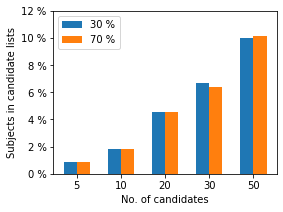
\includegraphics[width=\textwidth]{figures/supervised_approach/dropout_hw.png}
    \caption{Handwritten subjects}
    \label{fig:dropout_hw}
  \end{subfigure}
  \begin{subfigure}[t]{.32\textwidth}
    \centering
    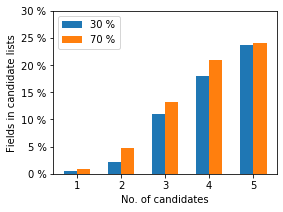
\includegraphics[width=\textwidth]{figures/supervised_approach/dropout_ddc.png}
    \caption{DDC subjects}
    \label{fig:dropout_ddc}
  \end{subfigure}
   \begin{subfigure}[t]{.32\textwidth}
    \centering
    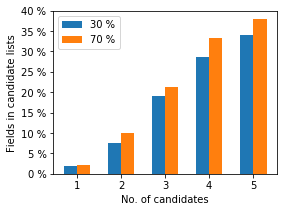
\includegraphics[width=\textwidth]{figures/supervised_approach/dropout_venue.png}
    \caption{Venues}
    \label{fig:dropout_venue}
  \end{subfigure}
  \caption{Model hit rate in the evaluation sets for different dropout probabilities.}
  \label{fig:dropout_eval}
\end{figure}

The dropout probability determines how likely it is for any element of the data to be zeroed. For instance, for a dropout probability of 50 \%, an element will be zeroed with 50 \% probability. Each element is considered independently of the rest.

In the original implementation, the authors use a dropout probability of 10 \%, which is rather low. The original proposers of dropout stated that a dropout of 50 \% is near optimal for many use cases \cite{srivastava2014dropout}. The approaches presented in chapter \ref{hmc}, which are also thematically similar to our approach, also used higher values: \cite{wehrmann2018hierarchical} uses 60 \% and \cite{giunchiglia2020coherent}, 70 \%.

For the authors of the original implementation, overfitting might not have been a threat, given that their data comprised over 11 million documents. In our case, with our smaller dataset, regularization is crucial. We therefore experiment with 50 \% and 70 \% dropout probability. Both models were trained with the same parameters, including a step-wise decaying learning rate scheduler. 

The losses during training, both throughout each epoch (figure \ref{fig:dropout_train_loss}) and on the test set (figure \ref{fig:dropout_test_loss}) are very similar during training. Although data was dropped twice as likely in one model than in the other, both models learned equally well according to the training data.

The accuracies of the models on the evaluation set are shown in figure \ref{fig:dropout_eval}. The model with less dropout seems to perform best for the handwritten subjects (figures \ref{fig:dropout_hw}), but only by a slight margin. The model with larger dropout probability performs considerably better in the other two evaluation sets, which consider the assignment of fields (figures \ref{fig:dropout_ddc} and \ref{fig:dropout_venue}, respectively).

A higher dropout probability seems to prevent overfitting, as the performance of both models is similar during training, but the one with more dropout performs better in the evaluation sets. We therefore use 70 \% as the dropout probability.

\subsubsection{Hidden layer size}

\begin{figure}
  \begin{subfigure}[t]{.5\textwidth}
    \centering
    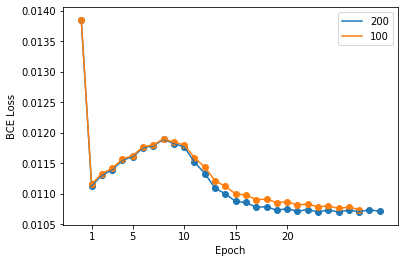
\includegraphics[width=\textwidth]{figures/supervised_approach/hidden_train_loss.png}
    \caption{Training loss}
    \label{fig:hidden_train_loss}
  \end{subfigure}
   \begin{subfigure}[t]{.5\textwidth}
    \centering
    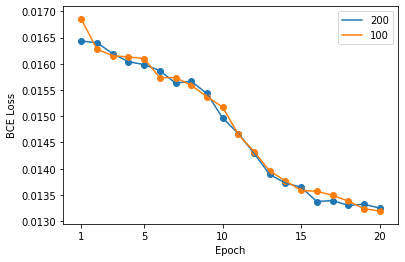
\includegraphics[width=\textwidth]{figures/supervised_approach/hidden_test_loss.png}
    \caption{Testing loss}
    \label{fig:hidden_test_loss}
  \end{subfigure}
  \caption{Test and training loss of models with different hidden layer sizes.}
  \label{fig:hidden_train}
\end{figure}

\begin{figure}
  \begin{subfigure}[t]{.32\textwidth}
    \centering
    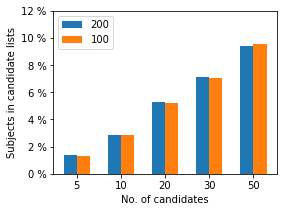
\includegraphics[width=\textwidth]{figures/supervised_approach/hidden_hw.png}
    \caption{Handwritten subjects}
    \label{fig:hidden_hw}
  \end{subfigure}
  \begin{subfigure}[t]{.32\textwidth}
    \centering
    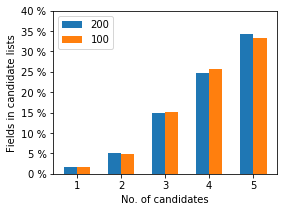
\includegraphics[width=\textwidth]{figures/supervised_approach/hidden_ddc.png}
    \caption{DDC subjects}
    \label{fig:hidden_ddc}
  \end{subfigure}
   \begin{subfigure}[t]{.32\textwidth}
    \centering
    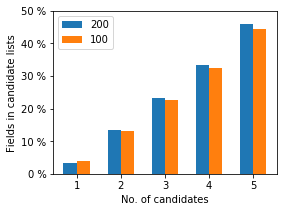
\includegraphics[width=\textwidth]{figures/supervised_approach/hidden_venue.png}
    \caption{Venues}
    \label{fig:hidden_venue}
  \end{subfigure}
  \caption{Model hit rate in the evaluation sets for different hidden layer sizes.}
  \label{fig:hidden_eval}
\end{figure}

The second parameter we experiment with is the size of the hidden layer, i.e. the size of the first fully connected layer. Its input is a one-dimensional vector of size 6,200, much smaller than the hidden layer input in the original implementation, which was over 20,000. More importantly, our set of subjects comprises 2,157 subjects, whereas the original implementation assigns 27.755 subjects to the documents. Their approach therefore requires more complexity than ours, and the hit rate of our model should not suffer with a smaller hidden layer size.

Furthermore, decreasing the complexity of the model further regularizes our pipeline, preventing overfitting. Given that the original implementation uses 1,024 nodes in the hidden layer and our set of subjects is one order of magnitude smaller than theirs, we experiment with hidden layer sizes of 100 and 200.

The training procedures are again very similar. As can be seen in figure \ref{fig:hidden_train}, both the training and testing losses of the different models are close to one another throughout all epochs. The evaluation results are also similar for both models, meaning that cutting the hidden layer size by half does not hinder the performance. Therefore, considering that the smaller size also alleviates the computational cost, we choose 100 as the hidden layer size.

\subsubsection{Learning rate schedule}

\begin{figure}
  \begin{subfigure}[t]{.5\textwidth}
    \centering
    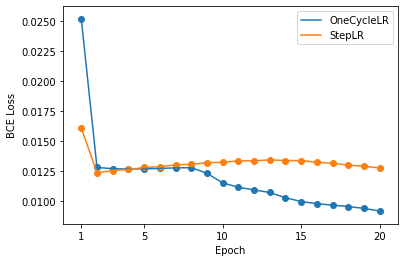
\includegraphics[width=\textwidth]{figures/supervised_approach/scheduler_train_loss.png}
    \caption{Training loss}
    \label{fig:scheduler_train_loss}
  \end{subfigure}
   \begin{subfigure}[t]{.5\textwidth}
    \centering
    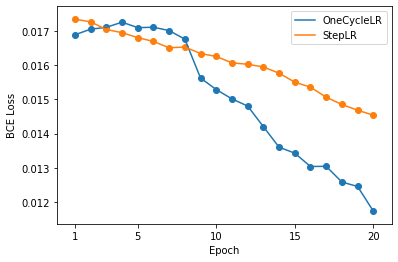
\includegraphics[width=\textwidth]{figures/supervised_approach/scheduler_test_loss.png}
    \caption{Testing loss}
    \label{fig:scheduler_test_loss}
  \end{subfigure}
  \caption{Test and training loss of models with different learning rate schedules.}
  \label{fig:scheduler_train}
\end{figure}

\begin{figure}
  \begin{subfigure}[t]{.32\textwidth}
    \centering
    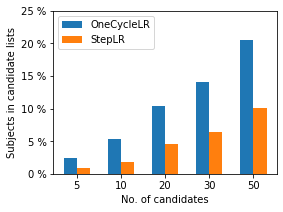
\includegraphics[width=\textwidth]{figures/supervised_approach/scheduler_hw.png}
    \caption{Handwritten subjects}
    \label{fig:scheduler_hw}
  \end{subfigure}
  \begin{subfigure}[t]{.32\textwidth}
    \centering
    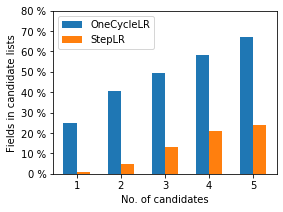
\includegraphics[width=\textwidth]{figures/supervised_approach/scheduler_ddc.png}
    \caption{DDC subjects}
    \label{fig:scheduler_ddc}
  \end{subfigure}
   \begin{subfigure}[t]{.32\textwidth}
    \centering
    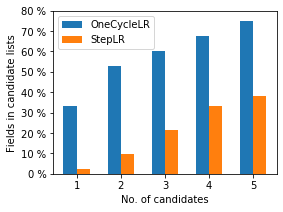
\includegraphics[width=\textwidth]{figures/supervised_approach/scheduler_venue.png}
    \caption{Venues}
    \label{fig:scheduler_venue}
  \end{subfigure}
  \caption{Model hit rate in the evaluation sets for different learning rate schedules.}
  \label{fig:scheduler_eval}
\end{figure}

\begin{figure}
    \centering
    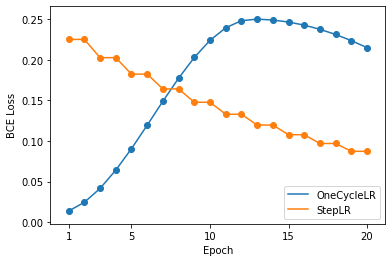
\includegraphics[width=.7\textwidth]{figures/supervised_approach/scheduler_lr.png}
    \caption{Learning rate schedules used in the experiments.}
    \label{fig:scheduler_lr}
\end{figure}

As mentioned at the beginning of this section, the original implementation uses a constant learning rate of $0.4$. Doing so is not common practice, as it is slower and does not necessarily reach optima as well as other procedures.

We have run the model with different constant learning rates to validate this assumption, and it holds: the models converge very slowly, taking small steps down the gradient, which lead to tiny loss improvements after every epoch. If we choose a higher constant learning rate, it soon starts overshooting the optimum, resulting in higher losses after a certain number of epochs.

We therefore try two learning rate schedules here. The first, called \textit{StepLR} in PyTorch, decreases the learning rate by 10 \% after every two epochs. This is the most intuitive approach: large steps are taken at the beginning, when the model is far away from its local optimal parameters. Once the model approaches the local optimum, the step size is decreased to not overshoot the optimum.

The second schedule follows the one-cycle policy, which is used in the paper where the asymmetric loss function is proposed \cite{ben2020asymmetric}. Cyclical learning rates \cite{smith2017cyclical} arise in the field of computer vision from the observation that increasing the learning rate may lead the model to perform better in the long term. The one-cycle policy, called \textit{OneCycleLR} in PyTorch, increases the learning rate until it reaches a given maximum, and then decreases it monotonically afterwards. The learning rate is updated multiple times during epochs.

Figure \ref{fig:scheduler_lr} shows both learning rate schedules across 20 epochs, both reaching a maximum learning rate of 0.25. The learning rate is updated every 100 batches in the one-cycle policy every 100 epochs, and every two epochs in the step-wise decay. The training procedures are very different from one another. The model trained with the step-wise schedule performs better in the test set (figure \ref{fig:scheduler_train_loss}) during the early epochs, where the learning rate of the one-cycle policy is still very low. However, after 10 epochs, the model trained with the one-cycle policy starts improving rapidly, being much more accurate than the other model in the end. A similar behavior can be seen in figure \ref{fig:scheduler_train_loss}, where the average training loss of each epoch is plotted.

As shown in figure \ref{fig:scheduler_eval}, the model with the one-cycle policy outperforms the one with the step-wise schedule by a very large margin, doubling its hit rate in all datasets. Especially when only one candidate is considered, it performs much better, given that the model trained with the step-wise schedule barely guesses and subjects or fields right. Thus, the three experiments we have performed show that a higher probability rate, a lower complexity and a cyclical learning rate perform best in our use case. The first two experiments indicate that regularization is important, given the differences between the documents of OpenAlex and those of the repositories.

\subsection{Asymmetric loss function} \label{hmc_asl}

\cite{ben2020asymmetric} addresses the imbalance between positive and negative labels in multi-label settings with an \acrfull{asl} function that dynamically down-weights and hard-thresholds easy negative samples, while also discarding possibly mislabeled samples. Training the state-of-the-art models in computer vision with this loss function significantly outperforms previous methods. On ResNet101, the common architecture used for multi-label classification, the asymmetric loss improves previous results by more than 1 \%. The \acrshort{asl} is also popular for its robustness against noise, as it is better suited for modeling noise in \acrshort{mlc} settings \cite{zhao2021evaluating}. The choice of the loss function plays a key role on how the model handles noise \cite{karimi2020deep}.

\subsubsection{BCE and focal loss}

\acrfull{bce}, the most popular loss function in multi-label classification settings, treats every label the same. For example, in a one-label setting where the model outputs $p=0.7$, if the label is positive ($y=1$), the \acrshort{bce} loss would be $-log(0.7) = 0.4$. If negative ($y=0$), the \acrshort{bce} loss would be $-log(0.3) = 1.2$, i.e. larger than in the other case, as the predicted probability is further away from the true label. The problem with using \acrshort{bce} in a multi-label setting is that most of the true labels for any given input are usually negative. In our case, any document is assigned only a few of the available subjects.

$$ BCE = \frac{1}{K} \sum_{k=1}^K -y_k \cdot \log (p_k) - (1-y_k) \cdot \log (1-p_k) $$

\acrfull{fl} addresses this issue by weighting each label score in a way that model outputs that are further away from their true labels gain more importance, whereas the model outputs that are already close to their targets are weighted down. Returning to the previous example and setting $\gamma=1$, a model output of $0.7$ with a positive true label ($y=1$) would receive a \acrshort{fl} of $-0.3 \cdot log(0.7) = 0.1$, and with a negative label ($y=0$), the \acrshort{fl} would be $-0.7 \cdot log(0.3) = 0.8$.

If we compare the results of both losses, we see that the difference between the results is much larger when using the \acrshort{fl}: they differ by a factor of 8 instead of by a factor of 3. The \acrshort{fl} gives more importance to the model output that was far away from its true label. Thus, the higher the \acrshort{fl} parameter $\gamma$ is set, the larger the difference will be between outputs that are close to their labels and those that are further away. However, setting $\gamma$ too high could remove the gradients from the rare positive samples \cite{ben2020asymmetric}.

$$ FL_\gamma = \frac{1}{K} \sum_{k=1}^K -y_k \cdot (1-p_k)^\gamma \cdot \log (p_k) - (1-y_k)\cdot p_k^\gamma \cdot \log (1-p_k) $$

\subsubsection{Asymmetric loss}

\acrfull{asl} overcomes this issue by decoupling the $\gamma$ parameter for negative and positive true labels, i.e. into $\gamma_-$ and $\gamma_+$, respectively. Setting $\gamma_- > \gamma_+$ emphasizes the contribution of positive samples, while giving less importance to negative samples that are close to their true label. Each of these three loss functions is an extension of the previous one. \acrshort{fl} equals \acrshort{bce} for $\gamma=0$, and \acrshort{asl} equals \acrshort{fl} for $\gamma_- = \gamma_+$.

$$ ASL_{\gamma_-,\gamma_+} = \frac{1}{K} \sum_{k=1}^K -y_k \cdot (1-p_k)^{\gamma_+} \cdot \log (p_k) - (1-y_k)\cdot p_k^{\gamma_-} \cdot \log (1-p_k) $$

The authors also propose using a hard threshold to discard negative samples below it, to further direct the training towards the positive samples. Although improving the performance of the models, this addition increases the complexity of the model, adding another parameter that requires tuning. They also experimented with dynamically tuning the $\gamma$ values, but concluded that doing so hindered the performance of the models. Still, they state this scheme could be useful for novice users.
\subsection{Coherence} \label{supervised_approach_coherence}

In this section, we implement the coherent model \cite{giunchiglia2020coherent}, which was explained in section \ref{hmc_forward}. Its contributions consist of a further layer after the model output, where the hierarchy is enforced upon the results, and a modification of the \acrfull{bce} loss function. Our initial model can thus be left intact, as we are only adding one last layer on top of it. This last layer, called \acrfull{mcm}, changes the assignment probability of each subject to be the maximum of its own probability and that of its descendants in the subject hierarchy. The formula can be found in section \ref{hmc_forward}.

We first discuss the implementation of the coherent model, and then run two experiments, where we combine the loss function of the coherent model, the \acrfull{mcl}, with the \acrfull{asl}.

\subsubsection{Implementation}

In practice, the \acrshort{mcm} is implemented as a matrix, where each row has ones for the subject it represents and its descendants, and zeros otherwise. Each row of this matrix is multiplied element-wise with the output of the model. Then, the maximum of each row is assigned to the corresponding subject. The \acrfull{mcl} modifies \acrshort{bce} loss to also ensure that the assignment probabilities respect the subject hierarchy, just as the \acrshort{mcm}. Thus, we can also extend it with the asymmetry between positive and negative samples, i.e. we can combine it with the \acrfull{asl}.

We therefore run two experiments. We first train this model with the \acrshort{mcl} as presented in the paper \cite{giunchiglia2020coherent}, and then run it again, with the \acrshort{mcl} combined with the ASL, i.e. the \acrfull{aml}. This means that the \acrshort{bce} is extended with the hierarchy constraints and also with the $\gamma$ parameters with which we weighted positive and negative samples in the previous section, as shown in the formula above.

\subsubsection{Experiments}

\begin{figure}
  \begin{subfigure}[t]{.5\textwidth}
    \centering
    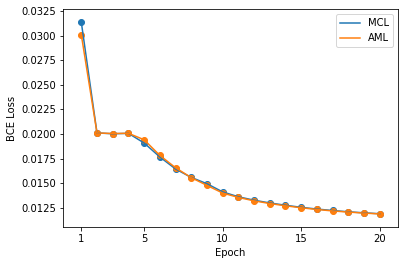
\includegraphics[width=\textwidth]{figures/supervised_approach/mcl_train_loss.png}
    \caption{Training loss}
    \label{fig:mcl_train_loss}
  \end{subfigure}
   \begin{subfigure}[t]{.5\textwidth}
    \centering
    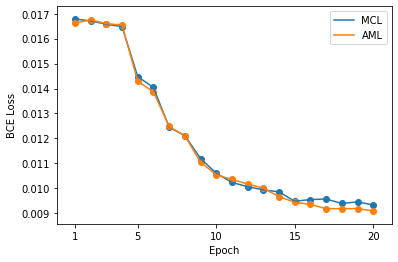
\includegraphics[width=\textwidth]{figures/supervised_approach/mcl_test_loss.png}
    \caption{Testing loss}
    \label{fig:mcl_test_loss}
  \end{subfigure}
  \caption{Test and training loss of coherent models with different gamma values.}
  \label{fig:mcl_train}
\end{figure}

\begin{figure}
  \begin{subfigure}[t]{.32\textwidth}
    \centering
    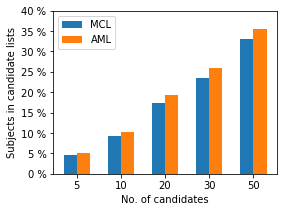
\includegraphics[width=\textwidth]{figures/supervised_approach/mcl_hw.png}
    \caption{Handwritten subjects}
    \label{fig:mcl_hw}
  \end{subfigure}
  \begin{subfigure}[t]{.32\textwidth}
    \centering
    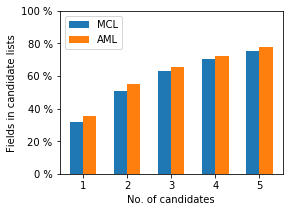
\includegraphics[width=\textwidth]{figures/supervised_approach/mcl_ddc.png}
    \caption{DDC subjects}
    \label{fig:mcl_ddc}
  \end{subfigure}
   \begin{subfigure}[t]{.32\textwidth}
    \centering
    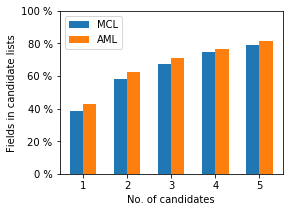
\includegraphics[width=\textwidth]{figures/supervised_approach/mcl_venue.png}
    \caption{Venues}
    \label{fig:mcl_venue}
  \end{subfigure}
  \caption{Hit rate of coherent models in the evaluation sets for different gamma values.}
  \label{fig:mcl_eval}
\end{figure}

The model used for these experiments is the same one as in section \ref{supervised_approach_asymmetric}, where we tested the asymmetric loss. The only difference is the addition of the \acrshort{mcm} layer on top of the model, and the different loss function. We have trained two models: one with the loss function from the paper \cite{giunchiglia2020coherent}, the \acrshort{mcl}, and one where the \acrshort{mcl} is combined with the \acrshort{asl}, which we call \acrfull{aml}. The parameters for the \acrshort{aml} are the ones that yielded the best results in our experiments with the \acrshort{asl}: $\gamma_+=1$ and $\gamma_-=2$.

As shown in figure \ref{fig:mcl_train}, the training procedures of both models are very similar. Both models start and end with similar training and testing losses, and also behave similarly throughout the 20 epochs both models were trained. However, the hit rate of the models on the evaluation sets favor the model trained with the \acrshort{aml}, which outscores its symmetric version for all evaluation sets and all number of candidates. The difference on the field evaluation sets is of 4 \% when only one candidate is considered, and of 2 \% on the handwritten evaluation set, when 50 candidates are considered. We therefore conclude that combining the \acrshort{asl} and \acrshort{mcl} yields the most accurate coherent model.
